\chapter{Opis techniczny}
Głównym tematem tego rozdziału jest opis techniczny wszystkich aplikacji i skryptów, które 
tworzą całe narzędzie. Została tu opisana struktura kodu i schemat komunikacji między 
aplikacjami.
Kod projektu można podzielić na cztery główne części:
\begin{enumerate}
  \item interfejs użytkownika,
  \item serwer komunikujący się z zewnętrznymi API oraz bazą danych,
  \item kod służący do instalacji zależności i uruchamiania aplikacji na maszynie wirtualnej 
  - korzystający z technologii Vagrant i Ansible,
  \item skrypt w języku Python konwertujący wstawki w języku \LaTeX\ do obrazów.
\end{enumerate}

\section{Serwer}
Kod serwera i inne pliki potrzebne do jego działania znajdują się w katalogu \texttt{forms-app}.

\subsection{Kod źródłowy}
Kod źródłowy serwera znajduje się w katalogu \texttt{src}. Serwer udostępnia kilka adresów,
pod którymi można się z nim komunikować używając protokołu http:
\begin{itemize}
  \item \texttt{GET /forms}: zwraca wszystkie formularze, które znajdują się w lokalnej
    bazie danych,
  \item \texttt{GET /forms/:id}: zwraca informacje o formularzu o podanym identyfikatorze,
  \item \texttt{POST /forms}: pod ten adres można wysłać formularz w kodowaniu JSON, żeby
    stworzyć nowy formularz Google,
  \item \texttt{PUT /forms/:id}: pod ten adres można wysłać zakodowany formularz w formacie
    JSON, żeby edytować formularz o podanym identyfikatorze; edytowany jest formularz
    w lokalnej bazie danych oraz formularz Google,
  \item \texttt{GET /forms/:id/answers}: zwraca wszystkie przesłane odpowiedzi,
  \item \texttt{GET /forms/:id/scores}: zwraca wszystkie ocenione przesłane odpowiedzi,
  \item \texttt{GET /forms/:id/scores}: przesyła plik EXCEL z ocenionymi przesłanymi 
    odpowiedziami,
  \item \texttt{DELETE /forms/:id}: usuwa formularz o podanym identyfikatorze z lokalnej bazy
    danych oraz usuwa wszystkie pytania z formularza Google, ale nie usuwa formularza z
    dysku Google.
\end{itemize}
Kod z konfiguracją tych adresów można znaleźć w pliku \texttt{src/server.js}. Aplikacja
z interfejsem użytkownika używa tych adresów, żeby komunikować się z serwerem.
Plik \texttt{formsFunctions.js} zawiera funkcje pomocnicze, które przykładowo tworzą
zapytania wysyłane do Google Forms API lub oceniają zamknięte pytania w przesłanych
odpowiedziach i konwertują je do formatów JSON lub EXCEL. Plik \texttt{jsonValidator.js}
zawiera walidator zakodowanych formularzy w formacie JSON, który jest dokładnie opisany
w pracy \ap. W katalogu \texttt{tex2png} znajduje się moduł, który służy do uruchamiania
skryptu w języku Python, który tworzy obrazki ze wstawkami w języku \LaTeX\ i udostępnia
je na serwisie Imgur.

\subsection{Google Forms API}
W poprzedniej wersji projekt korzystał z Google Apps Script. Część kodu oraz utworzone
formularze Google były przechowywane na jednym konkretnym koncie Google, którego ewentualna
zmiana byłaby bardzo skomplikowana. Było to niewygodne w użyciu, może niezbyt bezpieczne
oraz utrudniało rozwój narzędzia. Dlatego zdecydowałam się przepisać część komunikującą się
serwerami Google na kod wysyłający zapytania do Google Forms API. Google Forms API to niedawno
powstałe API, które w łatwy sposób pozwala zarządzać formularzami Google na dowolnym koncie
Google i jest wciąż dynamiczne rozwijane, więc w przyszłości można liczyć na dodanie do niego
wielu funkcjonalności, które pozwoliłoby na dalszy rozwój narzędzia.
Żeby korzystać z Google Forms API wystarczy założyć projekt w konsoli Google Cloud, co jest w pełni
darmowe dla każdej osoby posiadającej konto Google i jest dokładnie opisane w następnym rozdziale.
Następnie użytkownik może pozwolić aplikacji zarządzać formularzami na swoim dysku Google bez obaw, 
że ktokolwiek inny miałby do nich dostęp. Serwer wysyła do Google Forms API zapytania i dostaje
 odpowiedzi w formacie JSON. Na ten moment API pozwala zarządzać formularzami oraz
przesłanymi do nich odpowiedziami, co pozwala na napisanie naszego własnego sposobu oceniania tych
odpowiedzi. Google Forms API udostępnia automatyczne ocenianie, ale za każde pytanie można
dostać tylko zero albo maksymalną liczbę punktów, co jest niewystarczające. Chcielibyśmy móc
za każde pytanie przydzielić przykładowo połowę punktów, jeśli nie zostały zaznaczone wszystkie
poprawne odpowiedzi. W tej pracy udało się to zrealizować.

\subsubsection{Uwierzytelnianie i autoryzacja}
Proces uwierzytelniania i autoryzacji z Google przebiega w kilku krokach:
\begin{enumerate}
  \item uwierzytelnianie aplikacji: kiedy aplikacja się uruchomia, wysyła ona swoje
    dane uwierzytelniające do Google z informacją, że chciałaby mieć dostęp do 
    formularzy użytkowników Google,
  \item ekran zgody: Google zwraca ekran zgody, w którym użytkownik musi wybrać swoje
    konto Google i zgodzić się na to, że aplikacja będzie mogła zarządzać formularzami
    na tym koncie. Jeśli użytkownik to zrobi, aplikacja wysyła zapytanie do Google
    ze swoimi danymi uwierzytelniającymi w celu uzyskania tokena dostępu, którego
    będzie teraz używać, żeby uzyskać dostęp do wszystkich potrzebnych zasobów,
  \item przyznanie tokena dostępu: jeśli wszystko przejdzie pomyślnie, Google
    odeśle aplikacji żądany token dostępu. Token zawiera informacje o tym, do których
    zasobów aplikacja uzyskała dostęp, 
  \item dostęp do zasobów: aplikacja może teraz wysyłać zapytania do Google, w których
    może zarządzać odpowiednimi zasobami, w naszym przypadku formularzami i przesłanymi
    do nich odpowiedziami,
  \item odświeżanie tokena: tokeny mają czas ważności i jeśli on upłynie, aplikacja
    musi poprosić o odświeżony token, aby móc dalej działać.
\end{enumerate}
Uwierzytelnianie i autoryzacja w serwisach Google są dokładnie opisane
w ich dokumentacji.

\subsection{Lokalna baza danych}
Do narzędzia została dodana możliwość automatycznego ocenienia zamkniętych pytań w 
przesłanych odpowiedziach. Google zapamiętuje przesłane odpowiedzi w postaci:
\begin{figure}[H]
  \begin{lstlisting}[language=json,firstnumber=1]
{
  "questionId": string,
  "textAnswers": {
    "answers": [
    {
      "value": string
    }
  ]
  }
}
  \end{lstlisting}
\end{figure}
Formularze Google są tworzone z przesłanego do serwera zakodowanego w formacie JSON obiektu,
którego opis można znaleźć w rozdziale ,,Instrukcja użytkownika''.
Tworząc pytanie w formularzu, Google nadaje mu identyfikator i potem posługuje się nim
zwracając przesłane do formularza odpowiedzi. Dla każdego pytania zwraca jego identyfikator 
w polu \texttt{questionId} i odpowiedzi w tablicy \texttt{answers}. Trzeba było zatem dodać
jakiś sposób, który pozwalałby na rozpoznanie, które pytanie w przesłanych odpowiedziach od 
Google to pytanie w przesłanym zakodowanym formularzu od użytkownika. Prostym sposobem było
dodanie bazy danych, która pamiętałaby zakodowany formularz razem jego identyfikatorem 
na serwerach Google, identyfikatorami pytań oraz sposobem oceniania tych pytań. Serwer
używa małej, lokalnej bazy
danych \texttt{lowdb}. Tworzy ona pliki, w których przechowuje dane w formacie JSON.
W przypadku naszej aplikacji lowdb tworzy plik o nazwie \texttt{db.json} w katalogu 
\texttt{src/database}. Zakodowane formularze w bazie danych wyglądają następująco:

\begin{figure}[H]
  \begin{lstlisting}[language=json,firstnumber=1]
FormTemplate {
  id: string, // identyfikator formularza
  title: string, // nazwa formularza
  questions: QuestionTemplate[], // tablica z pytaniami
  description?: string, // opis
  startDate?: string, // start testu
  endDate?: string, // koniec testu
  responderUri: string, // adres formularza Google
}
  \end{lstlisting}
\end{figure}
\begin{figure}[H]
  \begin{lstlisting}[language=json,firstnumber=1]
QuestionTemplate {
  questionId?: string, // identyfikator pytania typu list, 
                       // checkBox lub text
  type: QuestionType,  // typ pytania
  text: string, // tekst pytania
  tex: boolean, // pytanie zawiera wstawki matematyczne, 
                // gdy pole wynosi true
  answers?: AnswerTemplate[], // tablica odpowiedzi do 
                              // pytania
  points?: number, // punkty dla pytania typu list
  pointsArray?: Array<number> // tablica z punktami dla 
                              // pytania typu grid
}
  \end{lstlisting}
\end{figure}
\begin{figure}[H]
  \begin{lstlisting}[language=json,firstnumber=1]
QuestionType {
  list,
  checkBox,
  grid,
  text,
}
  \end{lstlisting}
\end{figure}
\begin{figure}[H]
  \begin{lstlisting}[language=json,firstnumber=1]
AnswerTemplate {
  questionId?: string, // identyfikator pytania dla typu 
                       // grid
  text: string, // tekst odpowiedzi
  tex: boolean, // zawiera wstawki matematyczne, 
                // gdy pole wynosi true
  correct: boolean, // poprawna, gdy pole wynosi true
}
  \end{lstlisting}
\end{figure}

Pola oznaczone ,,?:'' to pola, którym można przypisać wartość null. 
Pytania różnych typów różnią się od siebie swoim kodowaniem, ale 
aby uprościć ich reprezentację, powstał jeden model mogący reprezentować
je wszystkie. Jedna z różnic polega na tym, że dla pytań typu grid to
odpowiedzi w schemacie formularza są tak naprawdę kolejnymi podpytaniami,
więc każde takie podpytanie ma swój własny identyfikator. Zatem ich 
identyfikatory są przechowywane w polu \texttt{questionId} w 
\texttt{AnswerTemplate}. Identyfikatory pozostałych typów pytań są 
przechowywane w \texttt{QuestionTemplate}. Kolejna różnica polega na tym,
że pole \texttt{points} odnosi się tylko do pytań typu list, a pole 
\texttt{pointsArray} dotyczy pytań checkBox i grid.
\newpage
Aplikacja automatycznie ocenia przesłane odpowiedzi w kilku krokach:
\begin{enumerate}
  \item pobiera przesłane odpowiedzi od Google,
  \item dla każdej przesłanej odpowiedzi sprawdza, czy czas przesłania jest poprawny - po 
    rozpoczęciu i przed zakończeniem testu,
  \item dla każdej przesłanej odpowiedzi:
    \begin{enumerate}
      \item identyfikuje, które odpowiedzi dotyczą którego pytania,
      \item sprawdza, czy odpowiedzi są poprawne,
      \item przydziela liczbę punktów zgodnie z wprowadzonym przez użytkownika sposobem
        oceniania, więcej w rozdziale ,,Instrukcja użytkownika'',
    \end{enumerate}
  \item opcjonalnie generuje plik EXCEL z listą osób, które wzięły udział w teście
    i~ ich wynikami.
\end{enumerate}

 
\subsection{Katalog assets}
Wszystkie obrazki z tekstem ze wstawkami w języku \LaTeX\ oraz wszystkie inne pliki, które
powstają podczas ich tworzenia są generowane w katalogu \texttt{assets}, dlatego ważne jest, żeby
go nie usuwać. Zawartość tego katalogu można usunąć (oprócz pliku \texttt{.gitignore}), ponieważ
wygenerowane obrazki są używane tylko podczas tworzenia lub edytowania formularza.

\subsection{Katalog src/credentials}
W tym katalogu należy umieścić dane uwierzytelniające projektu Google. Więcej informacji można
znaleźć w rozdziale ,,Instrukcja użytkownika''. Nie należy usuwać tego katalogu.

\subsection{Katalog src/excels}
W tym katalogu można znaleźć wygenerowane podczas oceniania pliki EXCEL z wynikami. Nie należy go
usuwać, ale jego zawartość już można.

\subsection{ESLint}
Do aplikacji serwera został dodany ESLint, który pomaga pisać przejrzysty kod i na bieżąco
analizuje kod i sprawdza, czy nie zawiera on błędów. To zachowanie można dowolnie edytować używając 
zasad udostępnionych przez to narzędzie. Zasady skonfigurowane dla tego projektu można znaleźć 
w pliku \texttt{.eslintrc.json}. W celu dokładniejszego zrozumienia, jak działa to narzędzie 
zachęcam do zapoznania się z dokumentacją.

\section{Skrypt w języku Python}

Głównym zadaniem skryptu jest generowanie obrazków ze wstawkami w języku \LaTeX \ i zostało
już to napisane w poprzedniej wersji narzędzia. W tej pracy rozwinęliśmy go, dodając do
niego wgrywanie utworzonych obrazków do serwisu Imgur oraz opcję generowania
obrazków, które będą odpowiedziami do pytania. Poprzednia wersja narzędzia pozwalała
wgrywać wygenerowane obrazki tylko w miejsce pytania w formularzu Google.

\subsection{Imgur API}
% nowy template odpowiedzi
Ważną częścią funkcjonalności narzędzia jest tworzenie pytań ze wstawkami w języku \LaTeX.
Jest to realizowane przez konwertowanie wstawek do obrazków, a następnie dodawanie ich do 
formularzy w miejscu pytania lub odpowiedzi. Jak zostało wspomniane wcześniej narzędzie
przestało korzystać z Google Apps Script i zamiast tego korzysta teraz z Google Forms API.
Wysyłając zapytania, które mają dodać pytanie do formularza z obrazkiem, Google Forms API
przyjmuje tylko zewnętrzne URL, z których może pobrać te obrazki. Nie da się ich
bezpośrednio przesłać razem z zapytaniem. Pojawił się, więc problem jak udostępnić te
obrazki do pobrania. Postanowiłam wykorzystać do tego Imgur i Imgur API. Skrypt w języku Python,
który można znaleźć w katalogu \texttt{src/tex2png}, tworzy obrazki, a następnie przesyła je 
do Imgur API, a z powrotem otrzymuje adresy, które serwer przesyła do Google Forms API.
Następnie Google pobiera obrazy z podanych adresów i dodaje pytanie do formularza Google.

\subsection{Pliki graficzne w odpowiedziach do pytań}
Kolejną dodaną do narzędzia funkcjonalnością jest możliwość generacji odpowiedzi do pytań
w formularzu ze wstawkami w języku \LaTeX. Poprzednio było to możliwe tylko dla treści samych
pytań, ponieważ Google Apps Script nie oferował takiej możliwości, natomiast Google Forms API 
już na to pozwala. Pojawił się za to inny problem. Formularze Google wyświetlają odpowiedzi,
które są plikami graficznymi
w dość niefortunny sposób:
\begin{figure}[H]
  \centering
   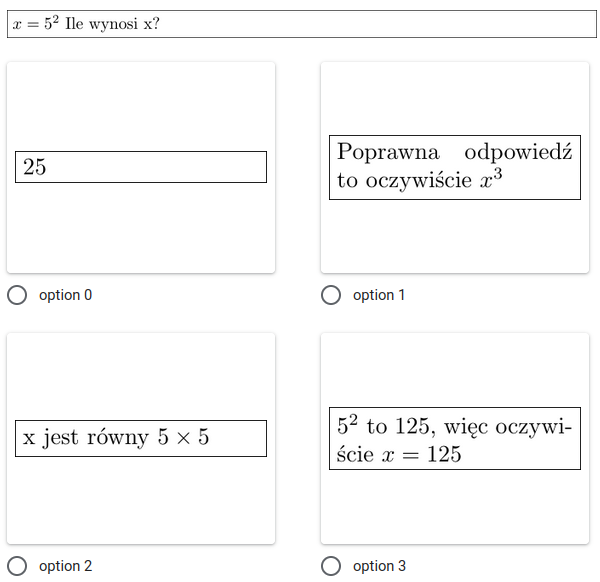
\includegraphics[scale=0.50]{odpowiedzi.png}
   \caption{Wygląd przykładowego formularza}
   \label{fig:1}
 \end{figure}
Dwie odpowiedzi zawsze zostaną umieszczona obok siebie, więc pliki graficzne z odpowiedziami
muszą być wąskie. Inaczej tekst odpowiedzi byłby bardzo mały. Zmiana wyświetlania odpowiedzi
z plikami graficznymi jest na ten moment niemożliwa. Dlatego do skryptu Google został dopisany
inny sposób generacji plików graficznych z odpowiedziami do pytań.

\section{Interfejs użytkownika}
Kod źródłowy aplikacji implementującej interfejs użytkownika znajduje się w katalogu
\texttt{forms-app-ui}. Aplikacja używa środowiska React i została stworzona używając programu
\texttt{Create React App}. Pliki \texttt{index.tsx} oraz \texttt{index.html}
tworzą podstawę całej aplikacji. W pliku \texttt{index.tsx} jest wstrzykiwany Reactowy
komponent \texttt{App}, który jest głównym komponentem całej aplikacji. W katalogu 
\texttt{src/components} można znaleźć wszystkie inne komponenty, które tworzą aplikację:
\begin{itemize}
  \item \texttt{FormCard}: implementuje jeden wpis z informacjami o formularzu,
  \item \texttt{FormList}: implementuje listę formularzy, czyli listę komponentów FormCard,
  \item \texttt{CreateDialog}: dialog, za pomocą którego można stworzyć nowy formularz,
  \item \texttt{AddDialog}: dialog, za pomocą którego można dodać już istniejący formularz,
  \item \texttt{EditDialog}: dialog, za pomocą którego można edytować formularz.
\end{itemize}
Aplikacja używa komponentów funkcyjnych oraz Reactowych hooków takich jak \texttt{useState},
\texttt{useEffect} i \texttt{useMemo}. W katalogu \texttt{src/models} znajdują się interfejsy
reprezentujące modele danych przesyłanych z serwera:
\begin{itemize}
  \item \texttt{AnswerTemplate}: jedna odpowiedź do pytania w formularzu,
  \item \texttt{QuestionTemplate}: jedno pytanie w formularzu,
  \item \texttt{FormTemplate}: formularz.
\end{itemize}
Dodatkowo znajduje się tam typ wyliczeniowy \texttt{QuestionType} z typami pytań.

\subsection{Material UI}
Implementacja korzysta z wiele komponentów z biblioteki Material UI takich jak:
\begin{itemize}
  \item \texttt{Alert} i \texttt{Collapse}, żeby wyświetlić ewentualne błędy,
  \item kontenery \texttt{List}, \texttt{ListItem}, \texttt{Box}, \texttt{Stack},
    \texttt{Accordion}, \texttt{Card},
  \item \texttt{Button}, żeby w łatwy sposób zaimplementować przyciski
    i ich logikę,
  \item \texttt{CircularProgress}, żeby wyświetlić animację ładowania, kiedy
    użytkownik musi poczekać na zakończenie jakiejś operacji,
  \item \texttt{Typography}, żeby wyświetlić tekst,
  \item \texttt{Dialog}, żeby zaimplementować dialogi,
  \item ikony.
\end{itemize}
Wszystkie te komponenty są niezwykle proste w użyciu oraz wyglądają przejrzyście
i łatwo do zrozumienia.
\subsection{Code Block}
Jeszcze jednym ważnym komponentem jest \texttt{CodeBlock} z biblioteki react-code-blocks.
Pozwala on łatwo wyświetlać fragmenty kodu razem z numerami linii i kolorowaniem
tekstu w zależności od języka kodu. Jest on wykorzystywany w komponencie FormCard.
\subsection{Daty}
Narzędzie pozwala określać rozpoczęcie i zakończenia testu, więc należało
zaimplementować zarządzanie datami. Aplikacja używa do tego biblioteki date-fns,
która jest lekka i prosta w użyciu. Przykładowo używamy funkcji \texttt{format}, żeby
ładnie wyświetlić daty we wpisach o formularzach.

\subsection{ESLint}
Podobnie jak w serwerze, tutaj również został użyty ESLint. W pliku
\texttt{.eslintrc.json}~zostały określone zasady dla projektu korzystającego
z języka TypeScript oraz środowiska React.

\section{Vagrant i Ansible}
Plik \texttt{Vagrantfile} służy do konfiguracji maszyny wirtualnej i środowiska,
na której będzie działać narzędzie. Wyjaśnię teraz krótko, jak działa ten 
skrypt. Pole \texttt{config.vm.box} określa jaki system operacyjny zostanie
użyty, w naszym przypadku jest to Ubuntu 20.04.4 LTS (Focal Fossa). 
Następnie skrypt instaluje Ansible i definiuje ścieżkę do playbooka Ansible,
który jest opisany w dalszej części tego rozdziału. W następnej części
udostępniamy porty na maszynie wirtualnej przez porty na systemie, na którym
działa ta maszyna.
\begin{verbatim}
  config.vm.network :forwarded_port, guest: 80, host: 8001
\end{verbatim}
W powyższym przykładzie udostępniamy port 8001 na maszynie wirtualnej
przez port 80 na systemie użytkownika. Dalej skrypt konfiguruje pamięć, którą
będzie mogła wykorzystać maszyna wirtualna i na końcu wypisuje wiadomość z adresami,
które należy odwiedzić po jej uruchomieniu. Przydatne polecenia:
\begin{itemize}
  \item \texttt{vagrant up}: uruchamia maszynę wirtualną,
  \item \texttt{vagrant halt}: zatrzymuje maszynę wirtualną,
  \item \texttt{vagrant reload}: resetuje maszynę wirtualną,
  \item \texttt{vagrant destroy}: usuwa maszynę wirtualną,
  \item \texttt{vagrant provision}: przeprowadza od początku proces konfiguracji
    maszyny razem z ponownym zainstalowaniem zależności z playbooka Ansible.
\end{itemize}

\subsection{Playbook}
Playbook to plik w formacie yaml, który określa jakie programy i biblioteki
powinny zostać zainstalowane oraz jakie usługi powinny zostać uruchomione po
uruchomieniu maszyny wirtualnej. Można go znaleźć w katalogu \texttt{playbooks}
pod nazwą \texttt{playbook.yaml}. Są w nim określone wszystkie programy
i biblioteki opisane w rozdziale ,,Środowisko'' oraz są w nim dodane polecenia
uruchomienia usług przez menadżera systemu \texttt{systemd}. Te usługi uruchamiają
aplikacje serwera oraz interfejsu użytkownika i ich konfigurację można znaleźć
odpowiednio w plikach \texttt{forms-app.service} i \texttt{forms-app-ui.service}.
